\section{Introduction Part 1: Workflow - Session view + arrangement view}
\begin{itemize}
    \item When you open Ableton the software there will be a little box in the lower left corner of the screen. When you hover your mouse at any button, text will appear in this lower left corner box, describing what the button does. 
        \begin{figure}[H]
            \centering
            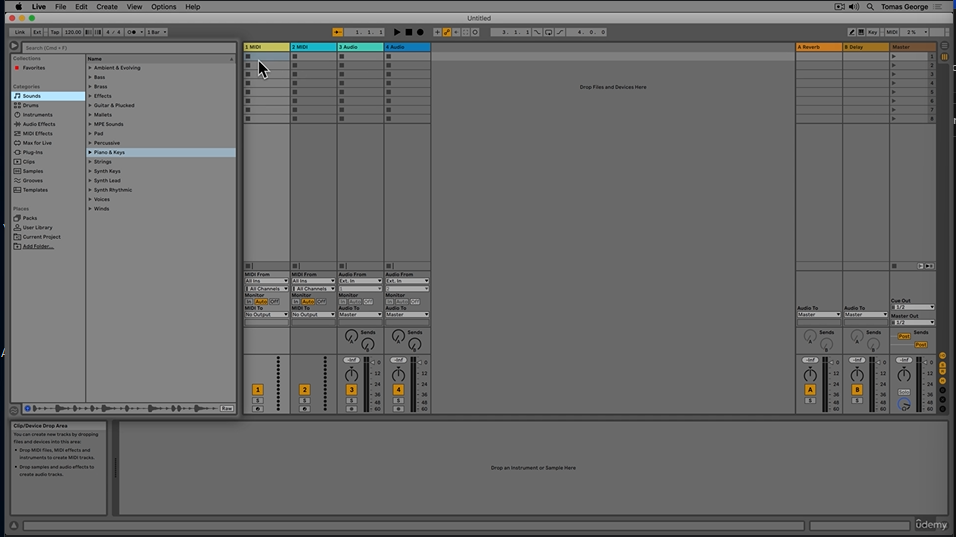
\includegraphics[width=\width\textwidth]{./figs/20220523171909.png}
            \caption{}
        \end{figure}

    \item On the top left we see the browser:
        \begin{figure}[H]
            \centering
            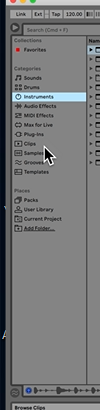
\includegraphics[width=\width\textwidth]{./figs/20220523171931.png}
            \caption{Browser}
        \end{figure}[H]
        \begin{itemize}
            \item The browser displays to you all the options you have, there is where you will find all the clips and tracks ready to go just to drag and drop.
        \end{itemize}
    
    \item There are two main views: session view and arrangement view. You can switch between them using the tab key.
        \begin{figure}[H]
            \centering
            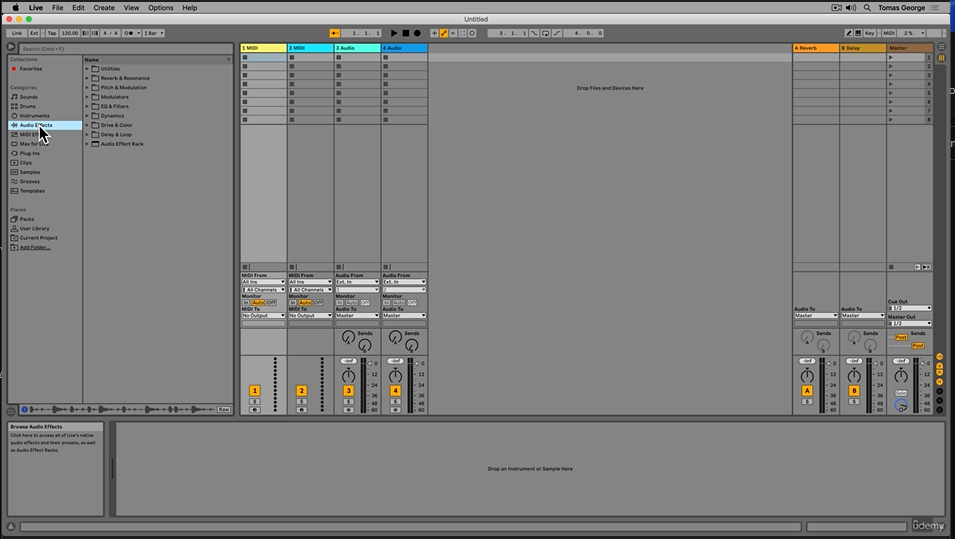
\includegraphics[width=\width\textwidth]{./figs/20220523172117.png}
            \caption{Session view}
        \end{figure}
        \begin{figure}[H]
            \centering
            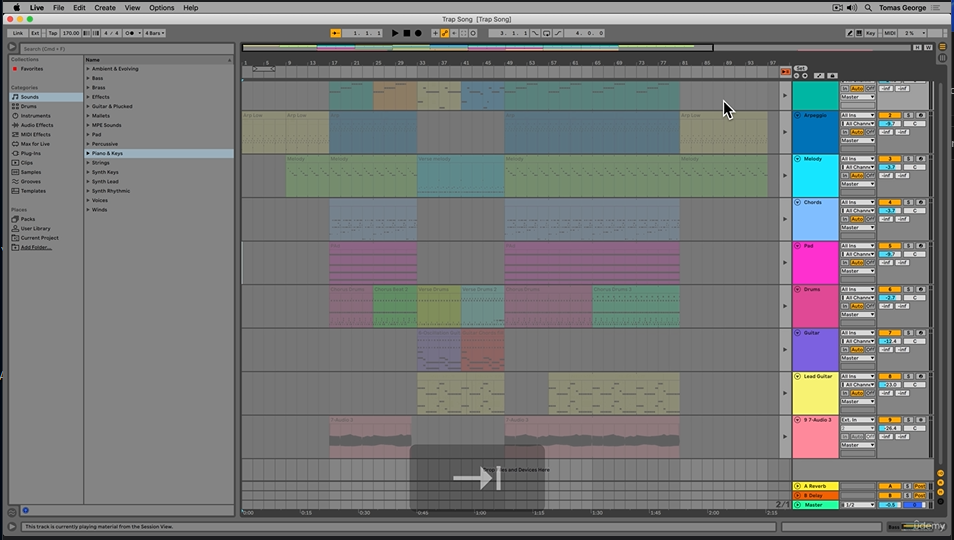
\includegraphics[width=\width\textwidth]{./figs/20220523172204.png}
            \caption{Arrangement view}
        \end{figure}

    
    \item Across the session view each of the columns are a separate track:
        \begin{figure}[H]
            \centering
            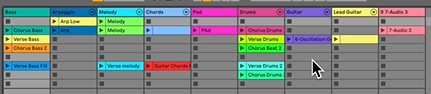
\includegraphics[width=\width\textwidth]{./figs/20220523172246.png}
            \caption{Tracks}
        \end{figure}
        \begin{itemize}
            \item We can have midi and audio tracks. 
        \end{itemize}
    
    \item Each of the squares in the following picture in the tracks is used to insert clips:
        \begin{figure}[H]
            \centering
            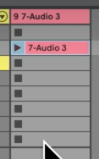
\includegraphics[width=\width\textwidth]{./figs/20220523172415.png}
            \caption{Adding clips}
        \end{figure}
    
    \item If you play the right most triangle then all the clips and midis in that row will play. This is known as a scene.
        \begin{figure}[H]
            \centering
            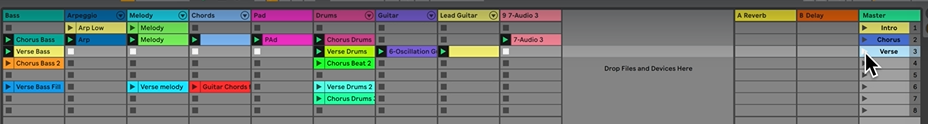
\includegraphics[scale=0.8]{./figs/20220523172505.png}
            \caption{Scenes}
        \end{figure}
    
    \item You can stop all clips with the 'stop all clips' button in the right midle part:
        \begin{figure}[H]
            \centering
            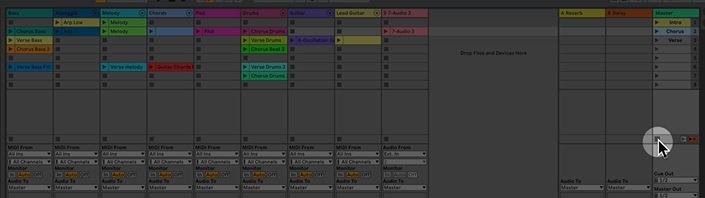
\includegraphics[]{./figs/20220523172604.png}
            \caption{Stop all clips}
        \end{figure}

    
    \item In the session view all of the tracks are listed vertically.
        \begin{figure}[H]
            \centering
            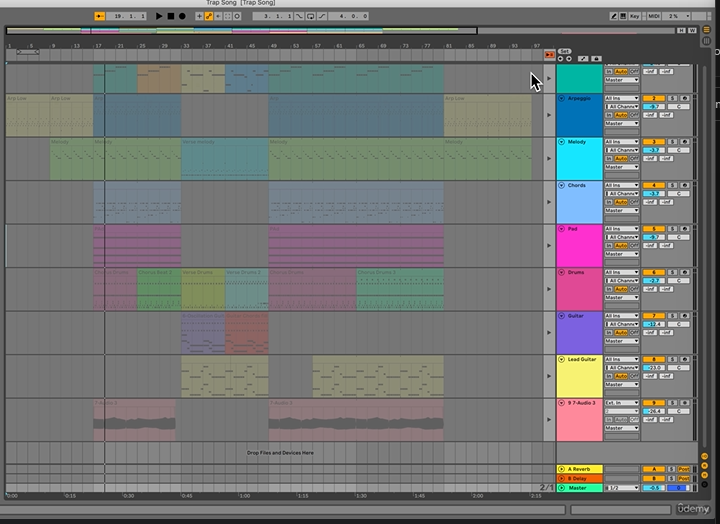
\includegraphics[width=\width\textwidth]{./figs/20220523172914.png}
            \caption{Session view's tracks}
        \end{figure}
    
        
    \item You can play and stop the tracks by pressing the space bar or pressing in the stop tracks button, which in session view looks like this:
        \begin{figure}[H]
            \centering
            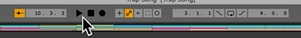
\includegraphics[width=\width\textwidth]{./figs/20220523173202.png}
            \caption{Stop all tracks}
        \end{figure}
    
    
    \item You can move the cursor to any point of the song by simply selecting it and moving it left or right.
        \begin{figure}[H]
            \centering
            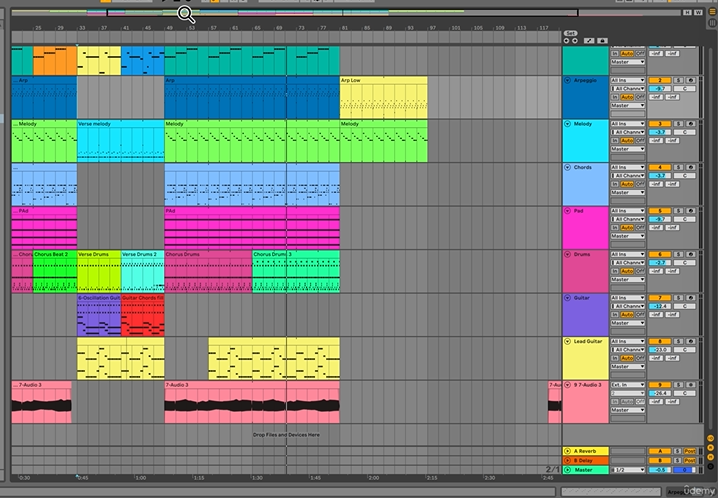
\includegraphics[width=\width\textwidth]{./figs/20220523173306.png}
            \caption{}
        \end{figure}
    
    \item The difference between session view and arrangement view is that the session view holds your musical ideas, and the arrangement view is used to structure your different ideas into a song.
    \item So the recomendation is to \textbf{come up with all of your musical ideas in the session view and structure them in the arrangement view}. This is not necesarry, but it is recomended.
\end{itemize}


\section{Introduction - Part 2: Creating clips}
\begin{itemize}
    \item Creating a clip can be as easy or as dificult as you require. You can pick an already made clip from the browser, or record your own clip and import it to ableton.
    \item Once you select a clip or sample you can simply click it and drag and drop it to a slot in the session view.
        \begin{figure}[H]
            \centering
            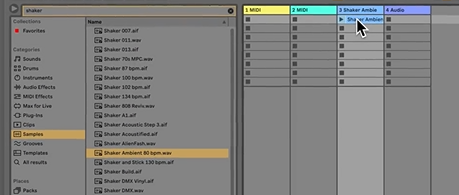
\includegraphics[width=\width\textwidth]{./figs/20220523174019.png}
            \caption{Clips drag and drop}
        \end{figure}
    
    \item By selecting the clip already in the clip slot we can see the wave form of the clip.
        \begin{figure}[H]
            \centering
            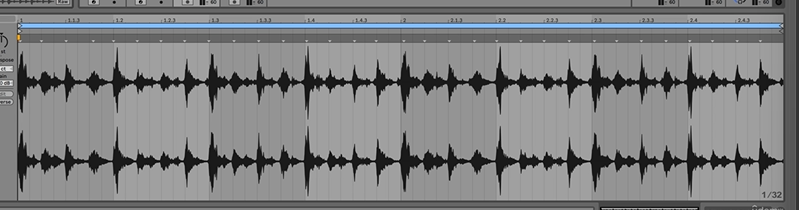
\includegraphics[width=\width\textwidth]{./figs/20220523174056.png}
            \caption{Waveform of the clip}
        \end{figure}
    
    \item Now lets open the midi column and insert a midi track, once we click on an empty slot in the midi track we see that the following is displayed:
        \begin{figure}[H]
            \centering
            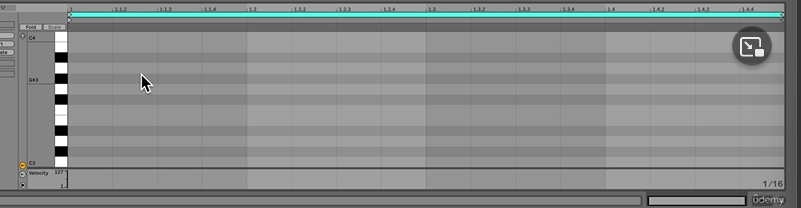
\includegraphics[width=\width\textwidth]{./figs/20220523174249.png}
            \caption{Midi}
        \end{figure}
    
    \item We can select which notes we want and create chords to our own song.
        \begin{figure}[H]
            \centering
            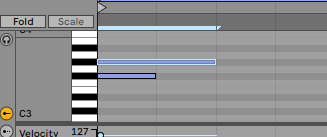
\includegraphics[width=\width\textwidth]{./figs/20220523174420.png}
            \caption{Midi note editor}
        \end{figure}
    
    \item You can adjust the note length by pressing the note: 
        \begin{figure}[H]
            \centering
            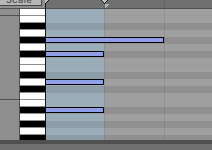
\includegraphics[width=\width\textwidth]{./figs/20220523174812.png}
            \caption{Note length}
        \end{figure}
    
    \item Notice that if you play it it does not actually make any sound. This is because midi tracks need an instument to create sound. We must load an instrument.
        \begin{itemize}
            \item Just go to the 'instruments' tab in your browser and select one. 
            \item Drag and drop it in the midi.
        \end{itemize}
        \begin{figure}[H]
            \centering
            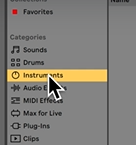
\includegraphics[width=\width\textwidth]{./figs/20220523174937.png}
            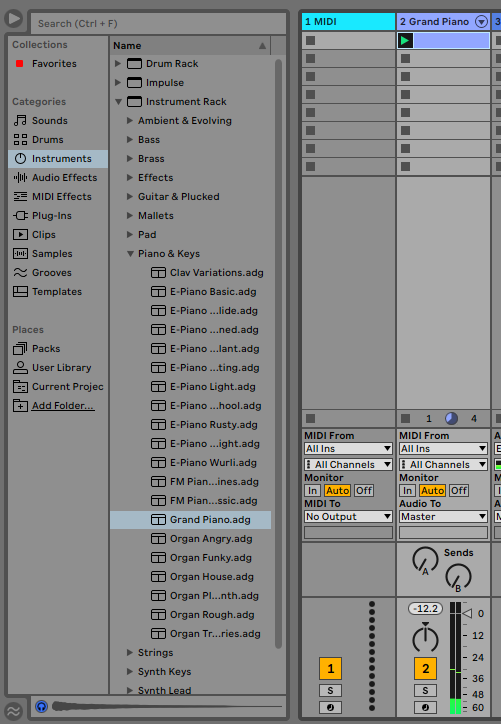
\includegraphics[width=\width\textwidth]{./figs/20220523175033.png}
            \caption{Adding an instrument to the midi track}
        \end{figure}
    
    \item Notice that the audio clips do not need an instrument to sound, this is because they are just audio. Whereas midi is more like instructions that need to be executed using an instrument.
    \item We can use all the available slots in the midi and clip columns to add as many sounds as you like.
    \item Now we record the clips to arrange them the arrangement view. Do this by pressing the red button and playing the tracks when you want them.
        \begin{figure}[H]
            \centering
            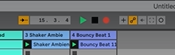
\includegraphics[width=\width\textwidth]{./figs/20220523175713.png}
            \caption{Recording}
        \end{figure}
    
    \item To tell ableton that we are done recording and we are now going to be arranging we press the following button:
        \begin{figure}[H]
            \centering
            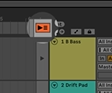
\includegraphics[width=\width\textwidth]{./figs/20220523175927.png}
            \caption{Back to arrangement button}
        \end{figure}
    
    \item Now we see our samples in the arrangement view:
        \begin{figure}[H]
            \centering
            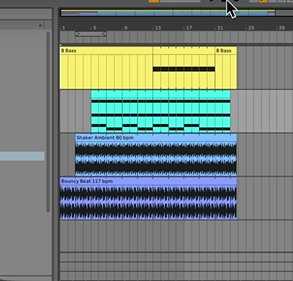
\includegraphics[width=\width\textwidth]{./figs/20220523175957.png}
            \caption{Arrangement view}
        \end{figure}
\end{itemize}

%%%%%%%%%%%%%%%%%%%%%%%%%%%%%%%%%%%%%%%%%%%%%%%%%%%%%%
\section{Introduction - Part 3: Basic Track Controls}
\begin{itemize}
    \item Once in arrangement view, if you ever need to listen to just one track and silence all the other onces there is a button for that called the solo track. It looks like this:
        \begin{figure}[H]
            \centering
            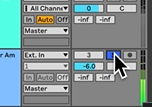
\includegraphics[width=\width\textwidth]{./figs/20220523180324.png}
            \caption{Solo track button}
        \end{figure}
    
    \item You can adjust the volume of a track by dragging the slider left or right:
        \begin{figure}[H]
            \centering
            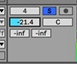
\includegraphics[width=\width\textwidth]{./figs/20220523180355.png}
            \caption{Adjusting track volume}
        \end{figure}
    
    \item We can adjust the panning of a track to adjust how far left or right it appears in the stereo image. Basically when you have 2 channels of sound sometimes you want sound to sound only in one channel rather than on 2. When you have earphones this is common, one sound only shows up in one side and not in both. This is to create an effect.
        \begin{figure}[H]
            \centering
            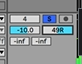
\includegraphics[width=\width\textwidth]{./figs/20220523180622.png}
            \caption{Panning}
        \end{figure}
    
    \item By double-clicking you restore the panning and the volume to default.
    \item By clicking on the orange track number shown below, we can mute that track:
        \begin{figure}[H]
            \centering
            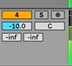
\includegraphics[width=\width\textwidth]{./figs/20220523180712.png}
            \caption{Muting one track}
        \end{figure}
    
    \item You can also access all of these controls in the session view. Here they are visually different but do the same things. Whatever you do in the session view will take effect in the arrangement view and vice-versa.
        \begin{figure}[H]
            \centering
            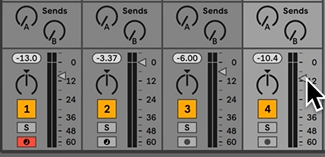
\includegraphics[width=\width\textwidth]{./figs/20220523180802.png}
            \caption{Session view controls}
        \end{figure}
\end{itemize}